% A fictional paper, made only to demonstrate Nomadys-PDF.
% pdflatex "\def\revised{1}% A fictional paper, made only to demonstrate Nomadys-PDF.
% pdflatex "\def\revised{1}% A fictional paper, made only to demonstrate Nomadys-PDF.
% pdflatex "\def\revised{1}% A fictional paper, made only to demonstrate Nomadys-PDF.
% pdflatex "\def\revised{1}\input{paper}" gives the revised version.
\documentclass[10pt,twocolumn]{article}
\usepackage[margin=1.8cm]{geometry}
\usepackage{amsmath,amssymb,graphicx,xcolor}
\usepackage{pgfplots}\pgfplotsset{compat=1.18}
\usepackage[colorlinks,linkcolor=blue!60!black,citecolor=green!45!black,urlcolor=blue!60!black]{hyperref}
\newcommand{\rev}[2]{\ifdefined\revised #2\else #1\fi}
\title{\bfseries Snap-through of bistable shells:\\ energy barriers, stiffness and control}
\author{A.~Nomad$^{1}$ \and B.~Traveller$^{2}$\\[2pt]
\small $^1$Institute of Soft Structures \quad $^2$Laboratory of Wandering Mechanics\\
\small \texttt{doi:10.5555/nomadys.demo.2026}}
\date{}
\begin{document}
\maketitle
\begin{abstract}
Bistable shells switch between two stable shapes through a snap-through
instability. We measure the energy barrier separating the two states, show
how the effective stiffness changes \rev{by a factor of 3.2}{by a factor of 3.7}
across the transition, and propose a simple strategy to control the switching
with a localized load. Our experiments agree with a reduced-order model within
\rev{8\%}{5\%}.
\end{abstract}

\section{Introduction}
Structures with more than one stable configuration are attractive for
deployable systems, morphing surfaces and mechanical memory
\cite{hu2015,holmes2019}. The key quantity is the energy barrier that separates
the stable states: it sets the load needed to switch and the robustness of each
state against disturbances \cite{gomez2017}. In this work we revisit the
snap-through of a clamped spherical cap, following the classical analysis of
\cite{koiter1945}, and relate the barrier to the measured stiffness.
Earlier studies focused on the load at which snap-through occurs, but the path between the two states matters as much: it determines how much energy is released, how fast the shell moves and whether the transition can be reversed. Here we combine a reduced-order model with full-field measurements to follow that path continuously, including the unstable branch that cannot be observed under load control.

\section{Model}
We describe the shell by the height $w(r)$ of its mid-surface. The elastic
energy combines bending and stretching,
\begin{equation}
  \mathcal{E} = \frac{B}{2}\int_\Omega (\nabla^2 w)^2\,\mathrm{d}A
  + \frac{Y}{2}\int_\Omega \varepsilon_{ij}\varepsilon_{ij}\,\mathrm{d}A ,
  \label{eq:energy}
\end{equation}
where $B = E t^3/12(1-\nu^2)$ is the bending stiffness and $Y = E t$ the
stretching stiffness. The snap-through load follows from the condition that
the tangent stiffness vanishes,
\begin{equation}
  k_t = \frac{\partial^2 \mathcal{E}}{\partial \delta^2} = 0 ,
  \label{eq:snap}
\end{equation}
which, for a shallow cap of rise $H$, gives a critical displacement
$\delta_c \approx \rev{0.62}{0.58}\,H$. Equation~\eqref{eq:energy} is minimised
numerically; the stability condition \eqref{eq:snap} identifies the limit
points shown in Fig.~\ref{fig:curve}.
The reduced-order model keeps the first two axisymmetric modes and one asymmetric mode. This is enough to capture both the symmetric limit point and the bifurcation to an asymmetric shape that occurs for deeper caps. The resulting energy landscape has two minima separated by a saddle, whose height we identify with the energy barrier. For the geometries tested here the barrier scales with the square of the rise, in agreement with the scaling expected for shallow shells.

\begin{figure}[t]
\centering
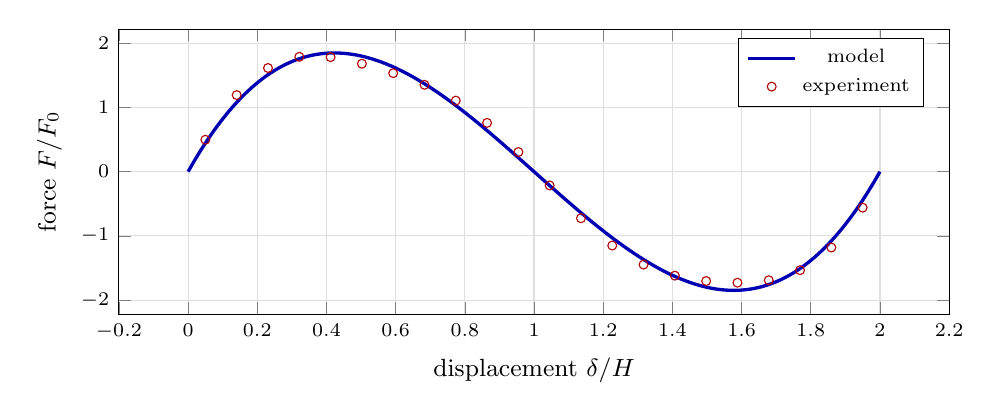
\begin{tikzpicture}
\begin{axis}[width=\columnwidth,height=5.2cm,xlabel={displacement $\delta/H$},
  ylabel={force $F/F_0$},grid=major,grid style={gray!25},legend pos=north east,
  legend style={font=\scriptsize},tick label style={font=\scriptsize},
  label style={font=\small}]
\addplot[very thick,blue!70!black,domain=0:2,samples=120]
  {3*x*(x-1)*(x-2)*1.6};
\addlegendentry{model}
\addplot[only marks,mark=o,red!70!black,mark size=1.6pt,domain=0.05:1.95,samples=22]
  {3*x*(x-1)*(x-2)*1.6 + 0.12*sin(deg(9*x))};
\addlegendentry{experiment}
\end{axis}
\end{tikzpicture}
\caption{Force--displacement response of the shell. The negative-stiffness
branch between the two limit points is unstable: under load control the shell
snaps through.}
\label{fig:curve}
\end{figure}

\section{Experiments}
The strain field during snap-through was measured with digital image
correlation (Fig.~\ref{fig:strain}). The maximum strain concentrates in a ring
at \rev{0.45}{0.41} of the radius, consistent with the model.
Each shell was clamped along its rim and loaded at its apex by a rigid indenter under displacement control, so that the unstable branch could be traced. The force was recorded at 1 kHz, and images were acquired simultaneously at 200 frames per second. The displacement field was reconstructed with a subset size of 31 pixels, giving a spatial resolution of about 0.4 mm on the shell surface.

\begin{figure}[t]
\centering
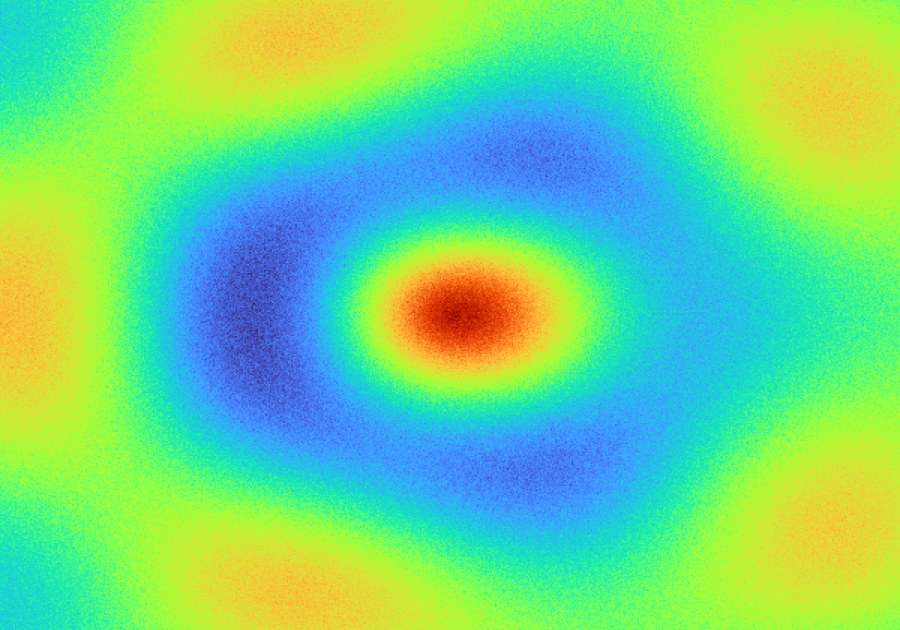
\includegraphics[width=\columnwidth]{strain.jpg}
\caption{Full-field strain map just before snap-through, measured by digital
image correlation.}
\label{fig:strain}
\end{figure}

\section{Stiffness across the transition}
The effective stiffness of the loaded shell drops to zero at the first limit
point and recovers after the snap. Table~\ref{tab:k} lists the values measured
for three thicknesses; the stiffness ratio grows with the thickness, as
predicted by Eq.~\eqref{eq:snap}.

\begin{table}[h]
\centering\small
\begin{tabular}{lccc}
\hline
thickness (mm) & $k_1$ (N/mm) & $k_2$ (N/mm) & ratio \\\hline
0.5 & 1.8 & 5.9 & 3.3\\
0.8 & 3.1 & \rev{10.2}{11.4} & \rev{3.3}{3.7}\\
1.2 & 5.6 & 19.8 & 3.5\\\hline
\end{tabular}
\caption{Stiffness before ($k_1$) and after ($k_2$) snap-through.}
\label{tab:k}
\end{table}
The stiffness ratio depends only weakly on the loading rate, which indicates that viscous effects in the elastomer play a minor role in the range tested. Close to the limit point, however, the response slows down markedly: the time needed to settle after a small load increment grows as the stiffness approaches zero, a signature of the critical slowing down reported for other elastic instabilities.

These observations suggest that the measured stiffness can be used as an early indicator of the approaching instability. In practical devices, monitoring the stiffness during actuation would allow the controller to anticipate the snap and to limit the energy released, which is useful when the shell carries sensitive components or must switch repeatedly without damage.

\section{Controlling the switch}
A localized load applied near the rim lowers the barrier by
\rev{40\%}{45\%}, so the shell can be switched with a small actuator
\cite{holmes2019}. We placed the localized load at three radial positions. Loading near the rim was the most effective, because it excites the asymmetric mode that provides the lowest path over the barrier. The switching force decreased accordingly, while the stability of each state against uniform pressure was unchanged, so the control does not compromise the robustness of the device.

\section{Conclusion}
Bistable shells offer a robust, tunable way to store mechanical states.
\rev{}{The revised measurements reduce the model error to 5\%. }
Future work will address arrays of coupled shells, in which the switching of one unit can trigger its neighbours, and the extension of the model to shells of non-uniform thickness, which offer additional freedom to shape the energy landscape.

\begin{thebibliography}{9}\small
\bibitem{koiter1945} W.~T. Koiter, \emph{On the stability of elastic
equilibrium}, PhD thesis, Delft (1945).
\bibitem{hu2015} N.~Hu and R.~Burgue\~no, Buckling-induced smart applications:
recent advances and trends, \emph{Smart Mater. Struct.} 24, 063001 (2015).
\bibitem{gomez2017} M.~Gomez, D.~E. Moulton and D.~Vella, Critical slowing down
in purely elastic snap-through instability, \emph{Nat. Phys.} 13, 142 (2017).
\bibitem{holmes2019} D.~P. Holmes, Elasticity and stability of shape-shifting
structures, \emph{Curr. Opin. Colloid Interface Sci.} 40, 118 (2019).
\end{thebibliography}
\end{document}
" gives the revised version.
\documentclass[10pt,twocolumn]{article}
\usepackage[margin=1.8cm]{geometry}
\usepackage{amsmath,amssymb,graphicx,xcolor}
\usepackage{pgfplots}\pgfplotsset{compat=1.18}
\usepackage[colorlinks,linkcolor=blue!60!black,citecolor=green!45!black,urlcolor=blue!60!black]{hyperref}
\newcommand{\rev}[2]{\ifdefined\revised #2\else #1\fi}
\title{\bfseries Snap-through of bistable shells:\\ energy barriers, stiffness and control}
\author{A.~Nomad$^{1}$ \and B.~Traveller$^{2}$\\[2pt]
\small $^1$Institute of Soft Structures \quad $^2$Laboratory of Wandering Mechanics\\
\small \texttt{doi:10.5555/nomadys.demo.2026}}
\date{}
\begin{document}
\maketitle
\begin{abstract}
Bistable shells switch between two stable shapes through a snap-through
instability. We measure the energy barrier separating the two states, show
how the effective stiffness changes \rev{by a factor of 3.2}{by a factor of 3.7}
across the transition, and propose a simple strategy to control the switching
with a localized load. Our experiments agree with a reduced-order model within
\rev{8\%}{5\%}.
\end{abstract}

\section{Introduction}
Structures with more than one stable configuration are attractive for
deployable systems, morphing surfaces and mechanical memory
\cite{hu2015,holmes2019}. The key quantity is the energy barrier that separates
the stable states: it sets the load needed to switch and the robustness of each
state against disturbances \cite{gomez2017}. In this work we revisit the
snap-through of a clamped spherical cap, following the classical analysis of
\cite{koiter1945}, and relate the barrier to the measured stiffness.
Earlier studies focused on the load at which snap-through occurs, but the path between the two states matters as much: it determines how much energy is released, how fast the shell moves and whether the transition can be reversed. Here we combine a reduced-order model with full-field measurements to follow that path continuously, including the unstable branch that cannot be observed under load control.

\section{Model}
We describe the shell by the height $w(r)$ of its mid-surface. The elastic
energy combines bending and stretching,
\begin{equation}
  \mathcal{E} = \frac{B}{2}\int_\Omega (\nabla^2 w)^2\,\mathrm{d}A
  + \frac{Y}{2}\int_\Omega \varepsilon_{ij}\varepsilon_{ij}\,\mathrm{d}A ,
  \label{eq:energy}
\end{equation}
where $B = E t^3/12(1-\nu^2)$ is the bending stiffness and $Y = E t$ the
stretching stiffness. The snap-through load follows from the condition that
the tangent stiffness vanishes,
\begin{equation}
  k_t = \frac{\partial^2 \mathcal{E}}{\partial \delta^2} = 0 ,
  \label{eq:snap}
\end{equation}
which, for a shallow cap of rise $H$, gives a critical displacement
$\delta_c \approx \rev{0.62}{0.58}\,H$. Equation~\eqref{eq:energy} is minimised
numerically; the stability condition \eqref{eq:snap} identifies the limit
points shown in Fig.~\ref{fig:curve}.
The reduced-order model keeps the first two axisymmetric modes and one asymmetric mode. This is enough to capture both the symmetric limit point and the bifurcation to an asymmetric shape that occurs for deeper caps. The resulting energy landscape has two minima separated by a saddle, whose height we identify with the energy barrier. For the geometries tested here the barrier scales with the square of the rise, in agreement with the scaling expected for shallow shells.

\begin{figure}[t]
\centering
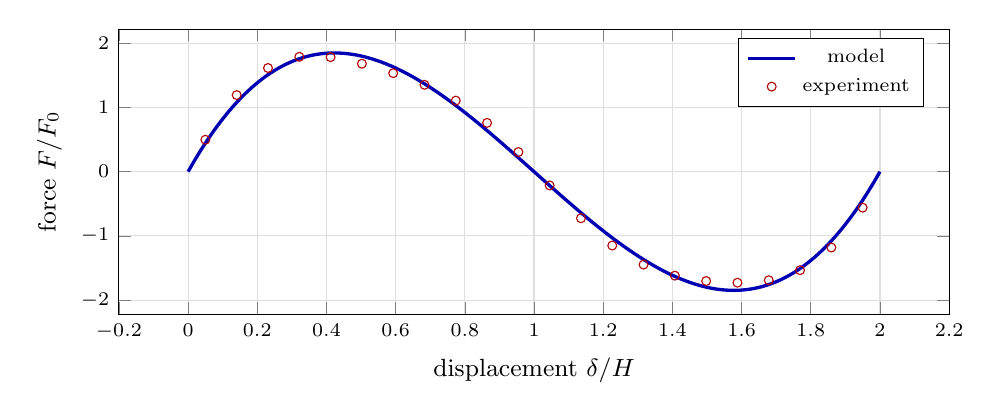
\begin{tikzpicture}
\begin{axis}[width=\columnwidth,height=5.2cm,xlabel={displacement $\delta/H$},
  ylabel={force $F/F_0$},grid=major,grid style={gray!25},legend pos=north east,
  legend style={font=\scriptsize},tick label style={font=\scriptsize},
  label style={font=\small}]
\addplot[very thick,blue!70!black,domain=0:2,samples=120]
  {3*x*(x-1)*(x-2)*1.6};
\addlegendentry{model}
\addplot[only marks,mark=o,red!70!black,mark size=1.6pt,domain=0.05:1.95,samples=22]
  {3*x*(x-1)*(x-2)*1.6 + 0.12*sin(deg(9*x))};
\addlegendentry{experiment}
\end{axis}
\end{tikzpicture}
\caption{Force--displacement response of the shell. The negative-stiffness
branch between the two limit points is unstable: under load control the shell
snaps through.}
\label{fig:curve}
\end{figure}

\section{Experiments}
The strain field during snap-through was measured with digital image
correlation (Fig.~\ref{fig:strain}). The maximum strain concentrates in a ring
at \rev{0.45}{0.41} of the radius, consistent with the model.
Each shell was clamped along its rim and loaded at its apex by a rigid indenter under displacement control, so that the unstable branch could be traced. The force was recorded at 1 kHz, and images were acquired simultaneously at 200 frames per second. The displacement field was reconstructed with a subset size of 31 pixels, giving a spatial resolution of about 0.4 mm on the shell surface.

\begin{figure}[t]
\centering
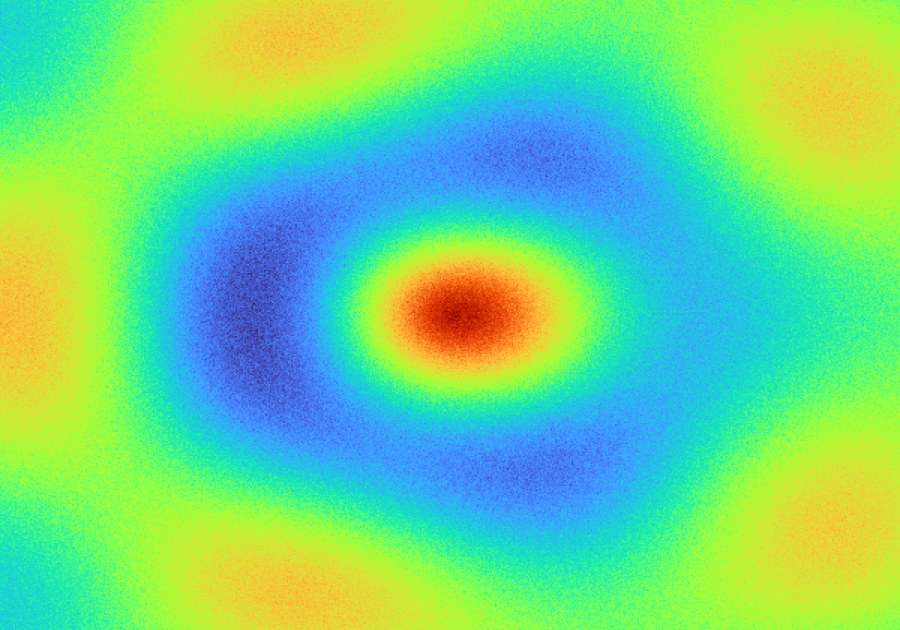
\includegraphics[width=\columnwidth]{strain.jpg}
\caption{Full-field strain map just before snap-through, measured by digital
image correlation.}
\label{fig:strain}
\end{figure}

\section{Stiffness across the transition}
The effective stiffness of the loaded shell drops to zero at the first limit
point and recovers after the snap. Table~\ref{tab:k} lists the values measured
for three thicknesses; the stiffness ratio grows with the thickness, as
predicted by Eq.~\eqref{eq:snap}.

\begin{table}[h]
\centering\small
\begin{tabular}{lccc}
\hline
thickness (mm) & $k_1$ (N/mm) & $k_2$ (N/mm) & ratio \\\hline
0.5 & 1.8 & 5.9 & 3.3\\
0.8 & 3.1 & \rev{10.2}{11.4} & \rev{3.3}{3.7}\\
1.2 & 5.6 & 19.8 & 3.5\\\hline
\end{tabular}
\caption{Stiffness before ($k_1$) and after ($k_2$) snap-through.}
\label{tab:k}
\end{table}
The stiffness ratio depends only weakly on the loading rate, which indicates that viscous effects in the elastomer play a minor role in the range tested. Close to the limit point, however, the response slows down markedly: the time needed to settle after a small load increment grows as the stiffness approaches zero, a signature of the critical slowing down reported for other elastic instabilities.

These observations suggest that the measured stiffness can be used as an early indicator of the approaching instability. In practical devices, monitoring the stiffness during actuation would allow the controller to anticipate the snap and to limit the energy released, which is useful when the shell carries sensitive components or must switch repeatedly without damage.

\section{Controlling the switch}
A localized load applied near the rim lowers the barrier by
\rev{40\%}{45\%}, so the shell can be switched with a small actuator
\cite{holmes2019}. We placed the localized load at three radial positions. Loading near the rim was the most effective, because it excites the asymmetric mode that provides the lowest path over the barrier. The switching force decreased accordingly, while the stability of each state against uniform pressure was unchanged, so the control does not compromise the robustness of the device.

\section{Conclusion}
Bistable shells offer a robust, tunable way to store mechanical states.
\rev{}{The revised measurements reduce the model error to 5\%. }
Future work will address arrays of coupled shells, in which the switching of one unit can trigger its neighbours, and the extension of the model to shells of non-uniform thickness, which offer additional freedom to shape the energy landscape.

\begin{thebibliography}{9}\small
\bibitem{koiter1945} W.~T. Koiter, \emph{On the stability of elastic
equilibrium}, PhD thesis, Delft (1945).
\bibitem{hu2015} N.~Hu and R.~Burgue\~no, Buckling-induced smart applications:
recent advances and trends, \emph{Smart Mater. Struct.} 24, 063001 (2015).
\bibitem{gomez2017} M.~Gomez, D.~E. Moulton and D.~Vella, Critical slowing down
in purely elastic snap-through instability, \emph{Nat. Phys.} 13, 142 (2017).
\bibitem{holmes2019} D.~P. Holmes, Elasticity and stability of shape-shifting
structures, \emph{Curr. Opin. Colloid Interface Sci.} 40, 118 (2019).
\end{thebibliography}
\end{document}
" gives the revised version.
\documentclass[10pt,twocolumn]{article}
\usepackage[margin=1.8cm]{geometry}
\usepackage{amsmath,amssymb,graphicx,xcolor}
\usepackage{pgfplots}\pgfplotsset{compat=1.18}
\usepackage[colorlinks,linkcolor=blue!60!black,citecolor=green!45!black,urlcolor=blue!60!black]{hyperref}
\newcommand{\rev}[2]{\ifdefined\revised #2\else #1\fi}
\title{\bfseries Snap-through of bistable shells:\\ energy barriers, stiffness and control}
\author{A.~Nomad$^{1}$ \and B.~Traveller$^{2}$\\[2pt]
\small $^1$Institute of Soft Structures \quad $^2$Laboratory of Wandering Mechanics\\
\small \texttt{doi:10.5555/nomadys.demo.2026}}
\date{}
\begin{document}
\maketitle
\begin{abstract}
Bistable shells switch between two stable shapes through a snap-through
instability. We measure the energy barrier separating the two states, show
how the effective stiffness changes \rev{by a factor of 3.2}{by a factor of 3.7}
across the transition, and propose a simple strategy to control the switching
with a localized load. Our experiments agree with a reduced-order model within
\rev{8\%}{5\%}.
\end{abstract}

\section{Introduction}
Structures with more than one stable configuration are attractive for
deployable systems, morphing surfaces and mechanical memory
\cite{hu2015,holmes2019}. The key quantity is the energy barrier that separates
the stable states: it sets the load needed to switch and the robustness of each
state against disturbances \cite{gomez2017}. In this work we revisit the
snap-through of a clamped spherical cap, following the classical analysis of
\cite{koiter1945}, and relate the barrier to the measured stiffness.
Earlier studies focused on the load at which snap-through occurs, but the path between the two states matters as much: it determines how much energy is released, how fast the shell moves and whether the transition can be reversed. Here we combine a reduced-order model with full-field measurements to follow that path continuously, including the unstable branch that cannot be observed under load control.

\section{Model}
We describe the shell by the height $w(r)$ of its mid-surface. The elastic
energy combines bending and stretching,
\begin{equation}
  \mathcal{E} = \frac{B}{2}\int_\Omega (\nabla^2 w)^2\,\mathrm{d}A
  + \frac{Y}{2}\int_\Omega \varepsilon_{ij}\varepsilon_{ij}\,\mathrm{d}A ,
  \label{eq:energy}
\end{equation}
where $B = E t^3/12(1-\nu^2)$ is the bending stiffness and $Y = E t$ the
stretching stiffness. The snap-through load follows from the condition that
the tangent stiffness vanishes,
\begin{equation}
  k_t = \frac{\partial^2 \mathcal{E}}{\partial \delta^2} = 0 ,
  \label{eq:snap}
\end{equation}
which, for a shallow cap of rise $H$, gives a critical displacement
$\delta_c \approx \rev{0.62}{0.58}\,H$. Equation~\eqref{eq:energy} is minimised
numerically; the stability condition \eqref{eq:snap} identifies the limit
points shown in Fig.~\ref{fig:curve}.
The reduced-order model keeps the first two axisymmetric modes and one asymmetric mode. This is enough to capture both the symmetric limit point and the bifurcation to an asymmetric shape that occurs for deeper caps. The resulting energy landscape has two minima separated by a saddle, whose height we identify with the energy barrier. For the geometries tested here the barrier scales with the square of the rise, in agreement with the scaling expected for shallow shells.

\begin{figure}[t]
\centering
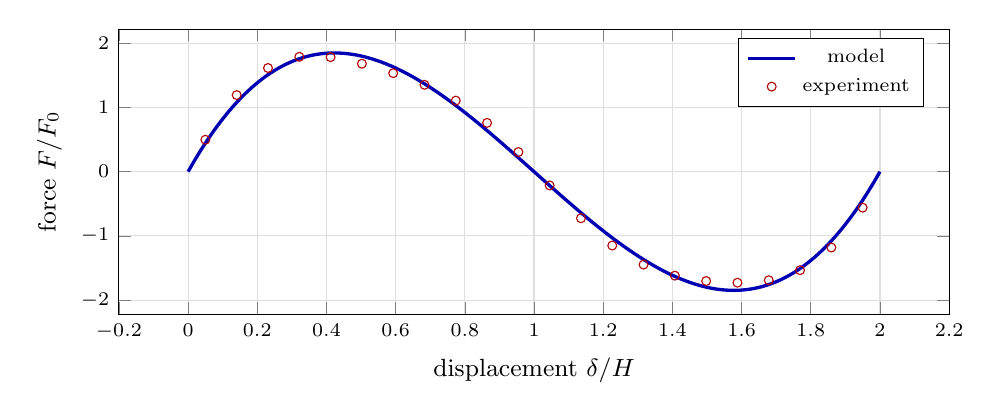
\begin{tikzpicture}
\begin{axis}[width=\columnwidth,height=5.2cm,xlabel={displacement $\delta/H$},
  ylabel={force $F/F_0$},grid=major,grid style={gray!25},legend pos=north east,
  legend style={font=\scriptsize},tick label style={font=\scriptsize},
  label style={font=\small}]
\addplot[very thick,blue!70!black,domain=0:2,samples=120]
  {3*x*(x-1)*(x-2)*1.6};
\addlegendentry{model}
\addplot[only marks,mark=o,red!70!black,mark size=1.6pt,domain=0.05:1.95,samples=22]
  {3*x*(x-1)*(x-2)*1.6 + 0.12*sin(deg(9*x))};
\addlegendentry{experiment}
\end{axis}
\end{tikzpicture}
\caption{Force--displacement response of the shell. The negative-stiffness
branch between the two limit points is unstable: under load control the shell
snaps through.}
\label{fig:curve}
\end{figure}

\section{Experiments}
The strain field during snap-through was measured with digital image
correlation (Fig.~\ref{fig:strain}). The maximum strain concentrates in a ring
at \rev{0.45}{0.41} of the radius, consistent with the model.
Each shell was clamped along its rim and loaded at its apex by a rigid indenter under displacement control, so that the unstable branch could be traced. The force was recorded at 1 kHz, and images were acquired simultaneously at 200 frames per second. The displacement field was reconstructed with a subset size of 31 pixels, giving a spatial resolution of about 0.4 mm on the shell surface.

\begin{figure}[t]
\centering
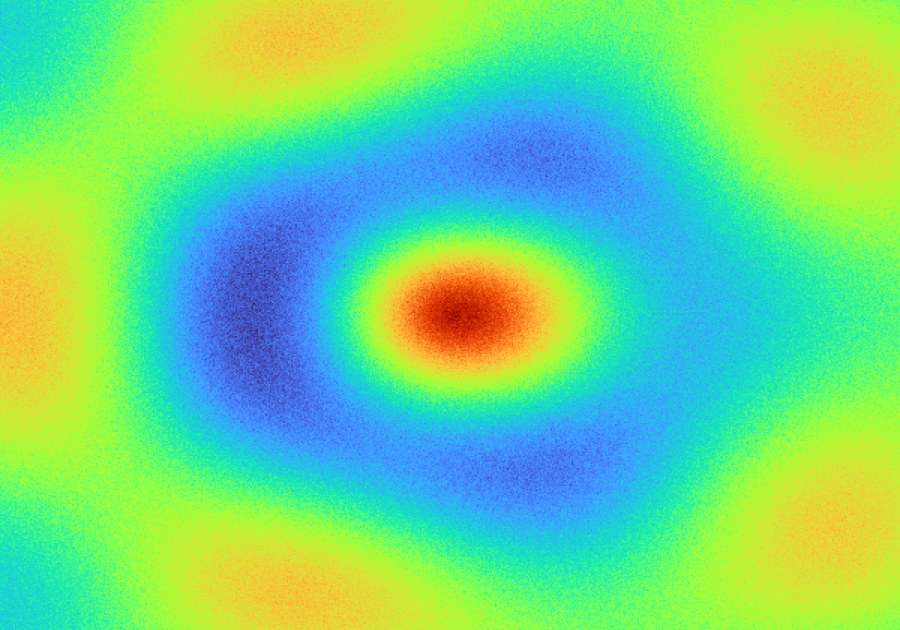
\includegraphics[width=\columnwidth]{strain.jpg}
\caption{Full-field strain map just before snap-through, measured by digital
image correlation.}
\label{fig:strain}
\end{figure}

\section{Stiffness across the transition}
The effective stiffness of the loaded shell drops to zero at the first limit
point and recovers after the snap. Table~\ref{tab:k} lists the values measured
for three thicknesses; the stiffness ratio grows with the thickness, as
predicted by Eq.~\eqref{eq:snap}.

\begin{table}[h]
\centering\small
\begin{tabular}{lccc}
\hline
thickness (mm) & $k_1$ (N/mm) & $k_2$ (N/mm) & ratio \\\hline
0.5 & 1.8 & 5.9 & 3.3\\
0.8 & 3.1 & \rev{10.2}{11.4} & \rev{3.3}{3.7}\\
1.2 & 5.6 & 19.8 & 3.5\\\hline
\end{tabular}
\caption{Stiffness before ($k_1$) and after ($k_2$) snap-through.}
\label{tab:k}
\end{table}
The stiffness ratio depends only weakly on the loading rate, which indicates that viscous effects in the elastomer play a minor role in the range tested. Close to the limit point, however, the response slows down markedly: the time needed to settle after a small load increment grows as the stiffness approaches zero, a signature of the critical slowing down reported for other elastic instabilities.

These observations suggest that the measured stiffness can be used as an early indicator of the approaching instability. In practical devices, monitoring the stiffness during actuation would allow the controller to anticipate the snap and to limit the energy released, which is useful when the shell carries sensitive components or must switch repeatedly without damage.

\section{Controlling the switch}
A localized load applied near the rim lowers the barrier by
\rev{40\%}{45\%}, so the shell can be switched with a small actuator
\cite{holmes2019}. We placed the localized load at three radial positions. Loading near the rim was the most effective, because it excites the asymmetric mode that provides the lowest path over the barrier. The switching force decreased accordingly, while the stability of each state against uniform pressure was unchanged, so the control does not compromise the robustness of the device.

\section{Conclusion}
Bistable shells offer a robust, tunable way to store mechanical states.
\rev{}{The revised measurements reduce the model error to 5\%. }
Future work will address arrays of coupled shells, in which the switching of one unit can trigger its neighbours, and the extension of the model to shells of non-uniform thickness, which offer additional freedom to shape the energy landscape.

\begin{thebibliography}{9}\small
\bibitem{koiter1945} W.~T. Koiter, \emph{On the stability of elastic
equilibrium}, PhD thesis, Delft (1945).
\bibitem{hu2015} N.~Hu and R.~Burgue\~no, Buckling-induced smart applications:
recent advances and trends, \emph{Smart Mater. Struct.} 24, 063001 (2015).
\bibitem{gomez2017} M.~Gomez, D.~E. Moulton and D.~Vella, Critical slowing down
in purely elastic snap-through instability, \emph{Nat. Phys.} 13, 142 (2017).
\bibitem{holmes2019} D.~P. Holmes, Elasticity and stability of shape-shifting
structures, \emph{Curr. Opin. Colloid Interface Sci.} 40, 118 (2019).
\end{thebibliography}
\end{document}
" gives the revised version.
\documentclass[10pt,twocolumn]{article}
\usepackage[margin=1.8cm]{geometry}
\usepackage{amsmath,amssymb,graphicx,xcolor}
\usepackage{pgfplots}\pgfplotsset{compat=1.18}
\usepackage[colorlinks,linkcolor=blue!60!black,citecolor=green!45!black,urlcolor=blue!60!black]{hyperref}
\newcommand{\rev}[2]{\ifdefined\revised #2\else #1\fi}
\title{\bfseries Snap-through of bistable shells:\\ energy barriers, stiffness and control}
\author{A.~Nomad$^{1}$ \and B.~Traveller$^{2}$\\[2pt]
\small $^1$Institute of Soft Structures \quad $^2$Laboratory of Wandering Mechanics\\
\small \texttt{doi:10.5555/nomadys.demo.2026}}
\date{}
\begin{document}
\maketitle
\begin{abstract}
Bistable shells switch between two stable shapes through a snap-through
instability. We measure the energy barrier separating the two states, show
how the effective stiffness changes \rev{by a factor of 3.2}{by a factor of 3.7}
across the transition, and propose a simple strategy to control the switching
with a localized load. Our experiments agree with a reduced-order model within
\rev{8\%}{5\%}.
\end{abstract}

\section{Introduction}
Structures with more than one stable configuration are attractive for
deployable systems, morphing surfaces and mechanical memory
\cite{hu2015,holmes2019}. The key quantity is the energy barrier that separates
the stable states: it sets the load needed to switch and the robustness of each
state against disturbances \cite{gomez2017}. In this work we revisit the
snap-through of a clamped spherical cap, following the classical analysis of
\cite{koiter1945}, and relate the barrier to the measured stiffness.
Earlier studies focused on the load at which snap-through occurs, but the path between the two states matters as much: it determines how much energy is released, how fast the shell moves and whether the transition can be reversed. Here we combine a reduced-order model with full-field measurements to follow that path continuously, including the unstable branch that cannot be observed under load control.

\section{Model}
We describe the shell by the height $w(r)$ of its mid-surface. The elastic
energy combines bending and stretching,
\begin{equation}
  \mathcal{E} = \frac{B}{2}\int_\Omega (\nabla^2 w)^2\,\mathrm{d}A
  + \frac{Y}{2}\int_\Omega \varepsilon_{ij}\varepsilon_{ij}\,\mathrm{d}A ,
  \label{eq:energy}
\end{equation}
where $B = E t^3/12(1-\nu^2)$ is the bending stiffness and $Y = E t$ the
stretching stiffness. The snap-through load follows from the condition that
the tangent stiffness vanishes,
\begin{equation}
  k_t = \frac{\partial^2 \mathcal{E}}{\partial \delta^2} = 0 ,
  \label{eq:snap}
\end{equation}
which, for a shallow cap of rise $H$, gives a critical displacement
$\delta_c \approx \rev{0.62}{0.58}\,H$. Equation~\eqref{eq:energy} is minimised
numerically; the stability condition \eqref{eq:snap} identifies the limit
points shown in Fig.~\ref{fig:curve}.
The reduced-order model keeps the first two axisymmetric modes and one asymmetric mode. This is enough to capture both the symmetric limit point and the bifurcation to an asymmetric shape that occurs for deeper caps. The resulting energy landscape has two minima separated by a saddle, whose height we identify with the energy barrier. For the geometries tested here the barrier scales with the square of the rise, in agreement with the scaling expected for shallow shells.

\begin{figure}[t]
\centering
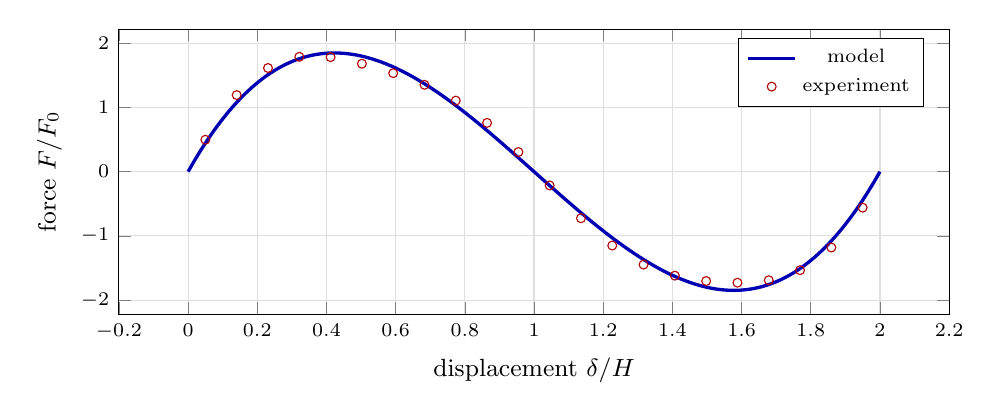
\begin{tikzpicture}
\begin{axis}[width=\columnwidth,height=5.2cm,xlabel={displacement $\delta/H$},
  ylabel={force $F/F_0$},grid=major,grid style={gray!25},legend pos=north east,
  legend style={font=\scriptsize},tick label style={font=\scriptsize},
  label style={font=\small}]
\addplot[very thick,blue!70!black,domain=0:2,samples=120]
  {3*x*(x-1)*(x-2)*1.6};
\addlegendentry{model}
\addplot[only marks,mark=o,red!70!black,mark size=1.6pt,domain=0.05:1.95,samples=22]
  {3*x*(x-1)*(x-2)*1.6 + 0.12*sin(deg(9*x))};
\addlegendentry{experiment}
\end{axis}
\end{tikzpicture}
\caption{Force--displacement response of the shell. The negative-stiffness
branch between the two limit points is unstable: under load control the shell
snaps through.}
\label{fig:curve}
\end{figure}

\section{Experiments}
The strain field during snap-through was measured with digital image
correlation (Fig.~\ref{fig:strain}). The maximum strain concentrates in a ring
at \rev{0.45}{0.41} of the radius, consistent with the model.
Each shell was clamped along its rim and loaded at its apex by a rigid indenter under displacement control, so that the unstable branch could be traced. The force was recorded at 1 kHz, and images were acquired simultaneously at 200 frames per second. The displacement field was reconstructed with a subset size of 31 pixels, giving a spatial resolution of about 0.4 mm on the shell surface.

\begin{figure}[t]
\centering
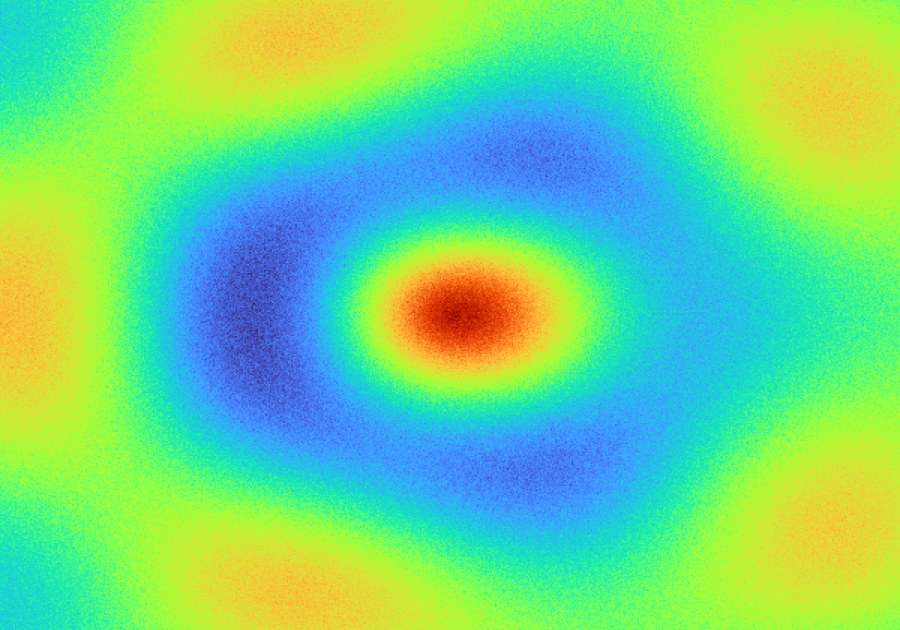
\includegraphics[width=\columnwidth]{strain.jpg}
\caption{Full-field strain map just before snap-through, measured by digital
image correlation.}
\label{fig:strain}
\end{figure}

\section{Stiffness across the transition}
The effective stiffness of the loaded shell drops to zero at the first limit
point and recovers after the snap. Table~\ref{tab:k} lists the values measured
for three thicknesses; the stiffness ratio grows with the thickness, as
predicted by Eq.~\eqref{eq:snap}.

\begin{table}[h]
\centering\small
\begin{tabular}{lccc}
\hline
thickness (mm) & $k_1$ (N/mm) & $k_2$ (N/mm) & ratio \\\hline
0.5 & 1.8 & 5.9 & 3.3\\
0.8 & 3.1 & \rev{10.2}{11.4} & \rev{3.3}{3.7}\\
1.2 & 5.6 & 19.8 & 3.5\\\hline
\end{tabular}
\caption{Stiffness before ($k_1$) and after ($k_2$) snap-through.}
\label{tab:k}
\end{table}
The stiffness ratio depends only weakly on the loading rate, which indicates that viscous effects in the elastomer play a minor role in the range tested. Close to the limit point, however, the response slows down markedly: the time needed to settle after a small load increment grows as the stiffness approaches zero, a signature of the critical slowing down reported for other elastic instabilities.

These observations suggest that the measured stiffness can be used as an early indicator of the approaching instability. In practical devices, monitoring the stiffness during actuation would allow the controller to anticipate the snap and to limit the energy released, which is useful when the shell carries sensitive components or must switch repeatedly without damage.

\section{Controlling the switch}
A localized load applied near the rim lowers the barrier by
\rev{40\%}{45\%}, so the shell can be switched with a small actuator
\cite{holmes2019}. We placed the localized load at three radial positions. Loading near the rim was the most effective, because it excites the asymmetric mode that provides the lowest path over the barrier. The switching force decreased accordingly, while the stability of each state against uniform pressure was unchanged, so the control does not compromise the robustness of the device.

\section{Conclusion}
Bistable shells offer a robust, tunable way to store mechanical states.
\rev{}{The revised measurements reduce the model error to 5\%. }
Future work will address arrays of coupled shells, in which the switching of one unit can trigger its neighbours, and the extension of the model to shells of non-uniform thickness, which offer additional freedom to shape the energy landscape.

\begin{thebibliography}{9}\small
\bibitem{koiter1945} W.~T. Koiter, \emph{On the stability of elastic
equilibrium}, PhD thesis, Delft (1945).
\bibitem{hu2015} N.~Hu and R.~Burgue\~no, Buckling-induced smart applications:
recent advances and trends, \emph{Smart Mater. Struct.} 24, 063001 (2015).
\bibitem{gomez2017} M.~Gomez, D.~E. Moulton and D.~Vella, Critical slowing down
in purely elastic snap-through instability, \emph{Nat. Phys.} 13, 142 (2017).
\bibitem{holmes2019} D.~P. Holmes, Elasticity and stability of shape-shifting
structures, \emph{Curr. Opin. Colloid Interface Sci.} 40, 118 (2019).
\end{thebibliography}
\end{document}
